Como se ha mencionado con anterioridad, el pedal tendrá una estructura en la que el primer paso es la captación de la señal para que pueda ser procesada. En este capítulo se detalla desde la elección del micrófono empleado hasta la salida de datos en formato adecuado para su interpretación por parte de la FPGA. Esta etapa es plenamente analógica, como suele suceder en otras etapas de amplificación de aparatos digitales.

\section{Captación de sonido: selección de micrófono}

Como normalmente se utilizan pedales de efectos en instrumentos electrófonos, la señal de salida del instrumento ya viaja por un cable de camino a la amplificador, por lo que el pedal actúa como un intermediario entre ambos. Sin embargo, en instrumentos de viento, es necesario utilizar un transductor que sea capaz de convertir la señal acústica consistente en ondas de presión en una serie de impulsos eléctricos que puedan ser debidamente interpretados posteriormente en la etapa digital.

La solución más sencilla consistiría en utilizar el micrófono que viene integrado con la placa Nexys A7: modelo \emph{ADMP421} de Analog Devices~\cite{Nexys}. No obstante, la utilización de este micrófono plantea los siguientes dos problemas.

En primer lugar, es inmediato pensar que incluso en el caso de un prototipo, si se plantea usar como pedal, no resulta nada recomendable colocar el micrófono encargado de recoger todo el sonido en el suelo. Además de estar lejos de la fuente sonora, capturaría el sonido resultante de la manipulación de los controles suponiendo una bajada en la calidad que proporcionase el dispositivo. Por tanto, es mejor utilizar un micrófono no integrado en la propia placa.

\begin{figure}
\begin{center}
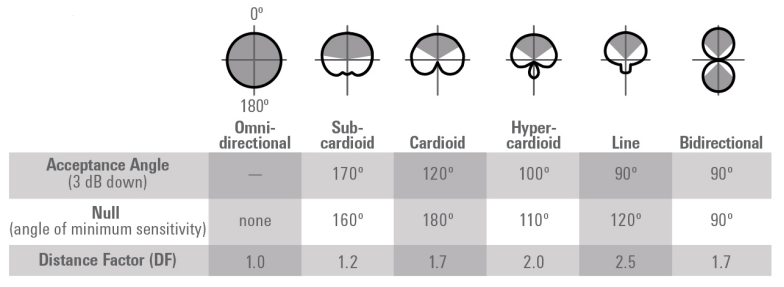
\includegraphics[width=15cm]{img/micros.png}
\caption{\label{fig:polar_dig}Tipos de micrófonos según su diagrama polar~\cite{Mic}}
\end{center}
\end{figure}

En segundo lugar, pero no menos importante, conviene tener en cuenta que la respuesta de sensibilidad del micrófono integrado es omnidireccional (ver figura \ref{fig:polar_dig}), es decir, captará todos los sonidos sin importar la dirección de dónde vengan. Este tipo de transductores se usan principalmente en radio y televisión, donde puede haber varias personas hablando en el mismo micrófono o para la grabación de orquestas o agrupaciones en localizaciones cerradas determinadas. Estos micrófonos son capaces de captar tanto el sonido proveniente de la fuente como los ecos y reflexiones característicos del espacio, dando una sensación de amplitud al oyente como la que produciría su escucha en esa misma localización. Pero mientras que en estos casos se trata de un efecto deseado, resulta poco agradable captar estas reflexiones en un ambiente no preparado para ello y encima cercano al suelo, siendo más conveniente utilizar micrófonos de tipo cardioide.

Estos micrófonos son los más utilizados con instrumentos de viento, ya que el sonido suele provenir de un punto concreto. Es preciso matizar que en el caso del saxofón, contra la creencia popular, el sonido no sale siempre por la campana del instrumento. El sonido proviene, por el contrario, de la llave abierta más próxima a la embocadura, que suele estar centrado respecto al cuerpo del instrumento. En consecuencia, no resulta conveniente acercar el micrófono mucho a la campana descuidando otras llaves. La figura \ref{fig:saxo} muestra un saxofón alto aunque hay varios instrumentos de la misma familia.

\begin{figure}[!b]
\begin{center}
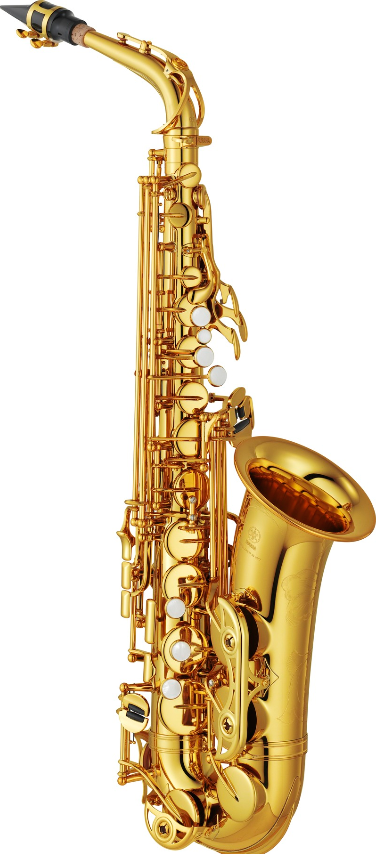
\includegraphics[height=8cm]{img/saxo.png}
\caption{\label{fig:saxo}Saxofón alto}
\end{center}
\end{figure}

Además de tener en cuenta el diagrama polar para la elección de micrófono, resulta imprescindible conocer los posibles tipos en cuanto a fabricación y funcionamiento. En este sentido se tendrán en cuenta los dos tipos más comunes: los micrófonos de condensador y los dinámicos los cuales se describen brevemente teniendo en cuenta el criterio de \emph{Shure}, uno de los fabricantes de audio profesional más reconocidos del mercado \cite{shuremic}.

Los micrófonos de condensador reciben su nombre del condensador que poseen en el interior de su cápsula. El diafragma es la pieza clave que se encarga de vibrar cuando las ondas de presión del sonido lo atraviesan. Esta pieza se une por uno de sus extremos con una de las placas del condensador. El resultado es que con cada movimiento del diafragma varía la distancia entre las placas y en consecuencia, se modifica la capacidad del conjunto de manera inversamente proporcional a las perturbaciones recibidas. Estos cambios modifican una señal eléctrica en la que quedan registradas las variaciones de las ondas de sonido recibidas. Estos micrófonos poseen una buena sensibilidad pero necesitan de alimentación \emph{phantom} de entre 24 y 48 V para polarizar el condensador, la cual se realiza desde la mesa de mezclas por el mismo cable de señal.

Los micrófonos dinámicos por el contrario, no requieren de alimentación \emph{phantom}, poseen buena robustez y son más baratos que los anteriores. Estos funcionan gracias a una bobina unida un diafragma similar al anterior que se mueve conforme a las ondas de presión recibidas del sonido dentro de un campo electromagnético creado por un imán. Por la acción de la inducción electromagnética se genera una corriente que atravesará la bobina de manera proporcional al estímulo entrante. La principal desventaja de estos micrófonos es que su respuesta no es del todo lineal con la frecuencia, produciendo mayor o menor ganancia en función del rango del espectro en el que se encuentre el sonido registrado. Para compensar este efecto se suele usar ecualización posterior o diferentes diafragmas para cada rango del espectro de forma que se pueda reconstruir la señal original a base de sumas de los diferentes tramos.

\begin{figure}[!hb]
\begin{center}
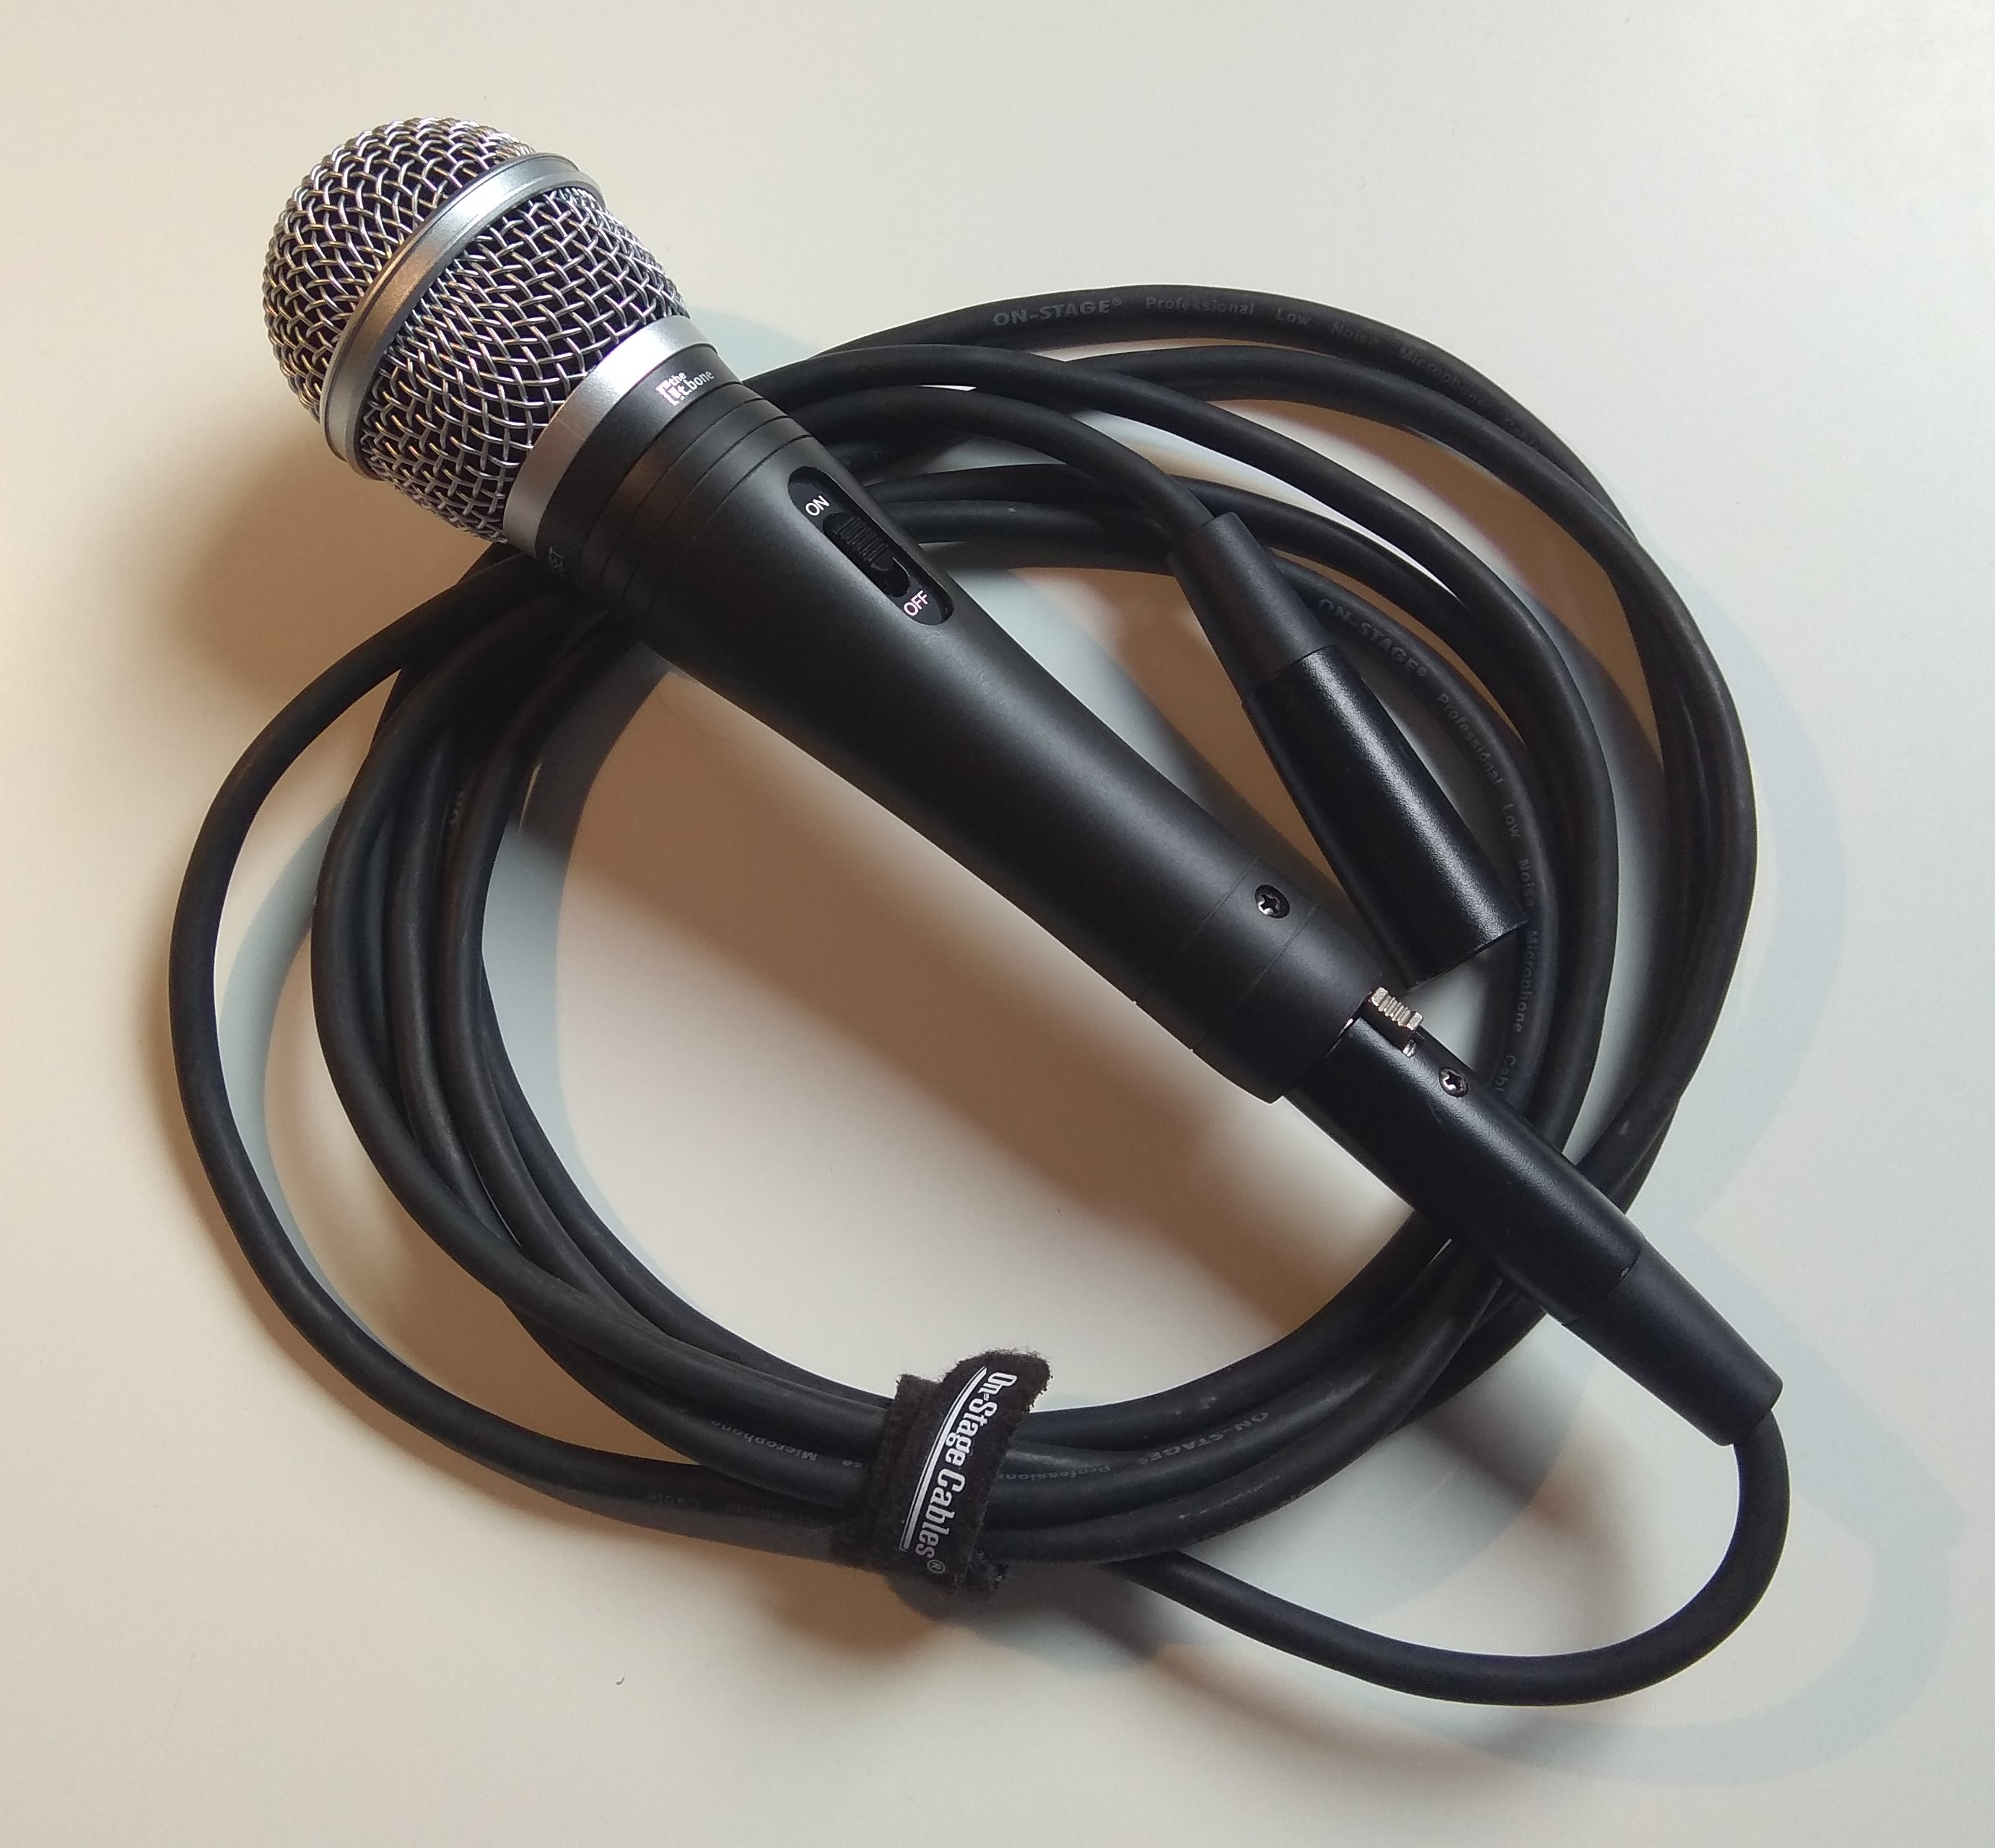
\includegraphics[width=8cm]{img/microusado.jpg}
\caption{\label{fig:microusado}Micrófono utilizado junto con el cable XLR}
\end{center}
\end{figure}

Teniendo en cuenta su uso en el diseño, he escogido un micrófono dinámico por la robustez que presenta que además evitará tener que preocuparse de la alimentación. Adicionalmente, estos micrófonos funcionan de manera muy similar entre sí, lo que resultará muy conveniente para mantener la flexibilidad del proyecto. El micrófono utilizado  finalmente en el prototipo será un \emph{T.Bone MB60} \cite{tbonemic} cortesía del Club Musical Delta, mostrado en la figura~\ref{fig:microusado}. El modelo elegido resulta increíblemente barato en comparación con sus rivales, sin embargo, su funcionamiento no resulta práctico para aplicaciones profesionales. Es evidente que ningún otro micrófono del mercado va a producir tanto ruido y poseer tantas no idealidades como este, por lo que resulta interesante para probar el prototipo en caso peor. El micrófono se colocará para capturar los sonidos en un pie en la ubicación más adecuada para el instrumento y se conectará a la etapa siguiente ubicada en el suelo mediante un cable XLR, del que se hablará más adelante.

En cualquier caso, es necesario añadir una etapa posterior de \emph{pre-amplificación}\footnote{Comúnmente se utiliza el término \emph{preamp} proveniente del inglés} que adecúe la señal eléctrica del micrófono a otra que pueda interpretar la FPGA. 

\section{Circuito analógico de previo o preamp}

La función principal que va a realizar este circuito será la de transformar la señal balanceada proveniente del micrófono en una sin balancear. Se realizará de manera puramente analógica aprovechando que el esquema está muy desarrollado en la literatura sobre el tema. En este caso he implementado el modelo propuesto por P.Allison en~\cite{Preamp}, el cual fue sugerido por el profesor Alfredo Sanz Hervás al que agradezco su referencia. En el mundo profesional, este tipo de circuitos recibe el nombre de \emph{previo} para micro o \emph{preamp} en inglés, debido a que siempre son necesarios para alimentar el micrófono empleado y adecuar su salida para su proceado o mezcla.

\begin{figure}[!htb]
\begin{center}
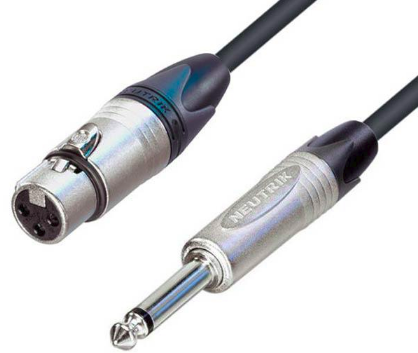
\includegraphics[width=6cm]{img/canonyjack.png}
\caption{\label{fig:conec}Conector tipo XLR hembra y jack no balanceado macho de 6.35 mm}
\end{center}
\end{figure}

Típicamente, los modelos de micrófonos comerciales para aplicaciones de música, utilizan conexiones balanceadas para proporcionar su señal a la salida. El formato de estos cables de 3 hilos recibe el nombre de \emph{XLR} pero también se pueden utilizar conectores de tipo \emph{Jack de 6.35 mm}\footnote{Este tipo de conector pero sin balancear, es el utilizado en guitarras y bajos eléctricos. Para los auriculares se utiliza jack de 3.5 mm que recibe el nombre de ``minijack''.} adecuados a este tipo de señales, ilustrados en la figura \ref{fig:conec}.

El funcionamiento del par balanceado consiste en enviar la señal por dos conductores entrelazados con la polaridad invertida entre sí, envueltos de un tercer conductor conectado a masa que actúa de barrera frente a interferencias electromagnéticas externas. Este proceso tiene sentido cuando se es capaz de recuperar la señal original rechazando las interferencias, para lo que se emplea un \emph{Amplificador de diferencias}\footnote{Traducción literal del inglés \emph{Difference Amplifier}, la traducción al castellano puede inducir a error} \cite{sfranco}, mostrado en la figura \ref{fig:adif}. 

\begin{figure}[!thb]
\begin{center}
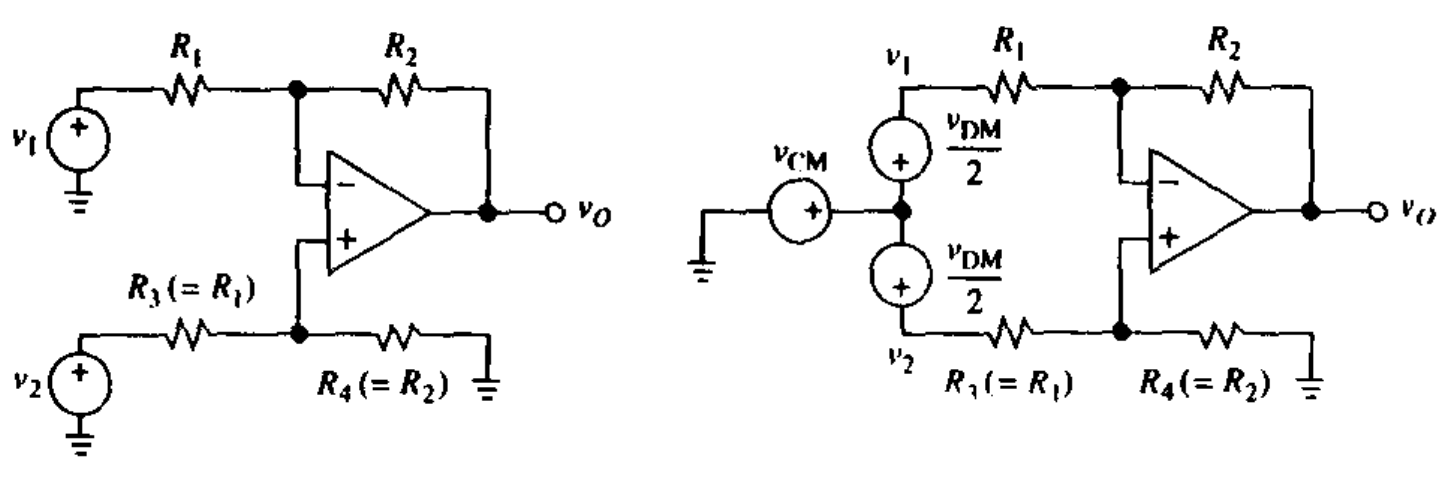
\includegraphics[width=13cm]{img/adiferencias.png}
\caption{\label{fig:adif}Amplificador de diferencias}
\end{center}
\end{figure}

Esta figura muestra la configuración de amplificador de diferencias basada en un amplificador operacional. La tensión de salida del circuito se puede escribir como:

\begin{equation}
\label{eq:Gnormal}
v_{o} = \dfrac{R_{2}}{R_{1}}(v_{2}-v_{1})
\end{equation}

Pero si cambiamos las expresiones de las tensiones de entrada según la ecuación \ref{eq:cambio} podemos reescribir el circuito, dando lugar a la segunda interpretación de la figura \ref{fig:adif}. En este caso $v_{MC}$ se interpreta como \emph{tensión en modo común} y $v_{MD}$ como la \emph{tensión en modo diferencial}.

\begin{equation}
\label{eq:cambio}
Si \begin{cases} v_{MD}=v_{2}-v_{1} \\ v_{MC}=\dfrac{v_{2}+v_{1}}{2}  \end{cases}~~~~Entonces \begin{cases} v_{1}=v_{MC}-v_{MD}/2 \\ v_{2}=v_{MC}+v_{MD}/2  \end{cases}
\end{equation}

El objetivo de este montaje es maximizar la ganancia para la entrada en modo diferencial rechazando el modo común, como figura en la ecuación \ref{eq:Gnormal}. Aunque idealmente, esto debería alcanzarse siempre, las características reales del operacional fuerzan que no se comporte exactamente de esta forma. Un pequeño desajuste en los valores reales de los resistores puede llegar a influir en gran manera en el funcionamiento del circuito. La manera de medir el comportamiento real de este proceso es mediante el CMRR, el factor de rechazo al modo común\footnote{Por sus siglas en inglés Common Mode Rejection Ratio}, mostrado en la ecuación \ref{eq:cmrr}, cuyo valor suele rondar los $100~dB$.

\begin{equation}
\label{eq:cmrr}
CMRR_{dB} = 20~log_{10}~\left |\frac{G_{MC}}{G_{MD}} \right |
\end{equation}

Volviendo a la conexión balanceada, es este rechazo al modo común el que permite eliminar las interferencias sufridas debido a que estas modifican la señal de igual manera en ambos conductores, al estar trenzados. Las componentes deseadas, al estar en contrafase, pertenecen al modo diferencial. Esta idea está muy extendida en los diseños analógicos de audio en entornos ruidosos, permitiendo enviar información por largos cables de manera robusta a cambio de introducir un tercer conductor. Esta etapa se corresponde con la zona amarilla de la figura \ref{fig:circuit}, que muestra el circuito completo tal y como figura en la bibliografía.

\begin{figure}[bht]
\begin{center}
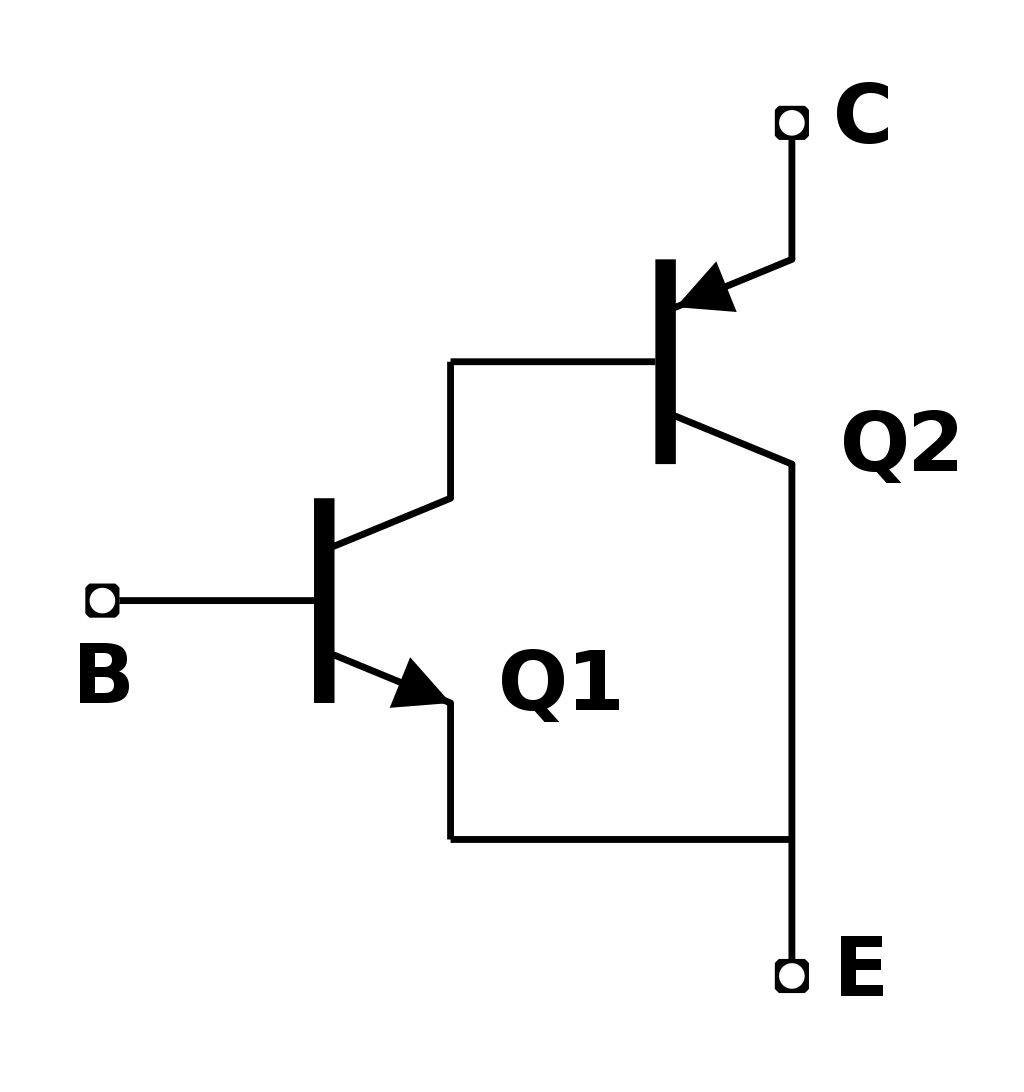
\includegraphics[width=4cm]{img/sziklai.png}
\caption{\label{fig:cfp}Configuración de dos transistores BJT en etapa CFP}
\end{center}
\end{figure}

La otra zona, la morada, se corresponde con una etapa de amplificación comúnmente utilizada en aplicaciones de audio \cite{ampaudio}. Esta consiste en una etapa CFP\footnote{Siglas en inglés de Complementary Feedback Pair, aunque en ocasiones recibe el nombre de Par Sziklai} para cada uno de los dos canales, junto con sus correspondientes resistencias de polarización. La característica fundamenteal de las etapas CFP es que el conjunto formado por transistor NPN y PNP, funciona en definitiva de forma equivalente a un único transistor NPN, ver figura \ref{fig:cfp}. Aproximadamente, la $\beta$ resultante en esta configuración, corresponde con el producto de los transistores BJT empleados, $\beta_{CFP}=\beta_{NPN}\cdot\beta_{PNP}$, lo que permite alcanzar una ganancia elevada. En este diseño se incluye un potenciómetro logarítmico que permite ajustar la ganancia de ambos canales a la vez controlando la polarización de ambas etapas CFP.

\begin{figure}[!thb]
\begin{center}
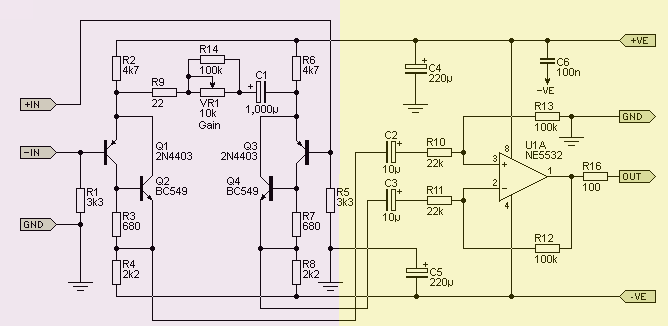
\includegraphics[width=13cm]{img/circuitochop.png}
\caption{\label{fig:circuit}Esquema del circuito de la etapa de entrada}
\end{center}
\end{figure}

La elección de los transistores y el amplificador operacional condiciona en gran medida el resultado obtenido: es importante que todos los componentes sean robustos frente al ruido. Además, la distorsión que introducen puede resultar más o menos agradable al oído. En consecuencia se ha seleccionado un operacional \emph{TL071} \cite{opampdata} por su bajo nivel de ruido y su reducido precio. Los transistores han sido de germanio, idénticos a los que propone P.Allison en su diseño.

También se incluyen condensadores de desacoplo en los terminales de alimentación que no se corresponden directamente con ninguna de las etapas descritas, pero en la figura~\ref{fig:circuit} se encuentran en la zona amarilla.

\section{Alimentación}
Para el correcto funcionamiento del circuito es necesario alimentar el operacional y proporcionar la corriente de polarización adecuada a los transistores. Aunque la bibliografía consultada es ambigua con este tema, finalmente se ha optado por utilizar una alimentación simétrica de $\pm15V$, que será proporcionada directamente de una fuente de alimentación del laboratorio (figura \ref{fig:fuente}). 

\begin{figure}[!hbt]
\begin{center}
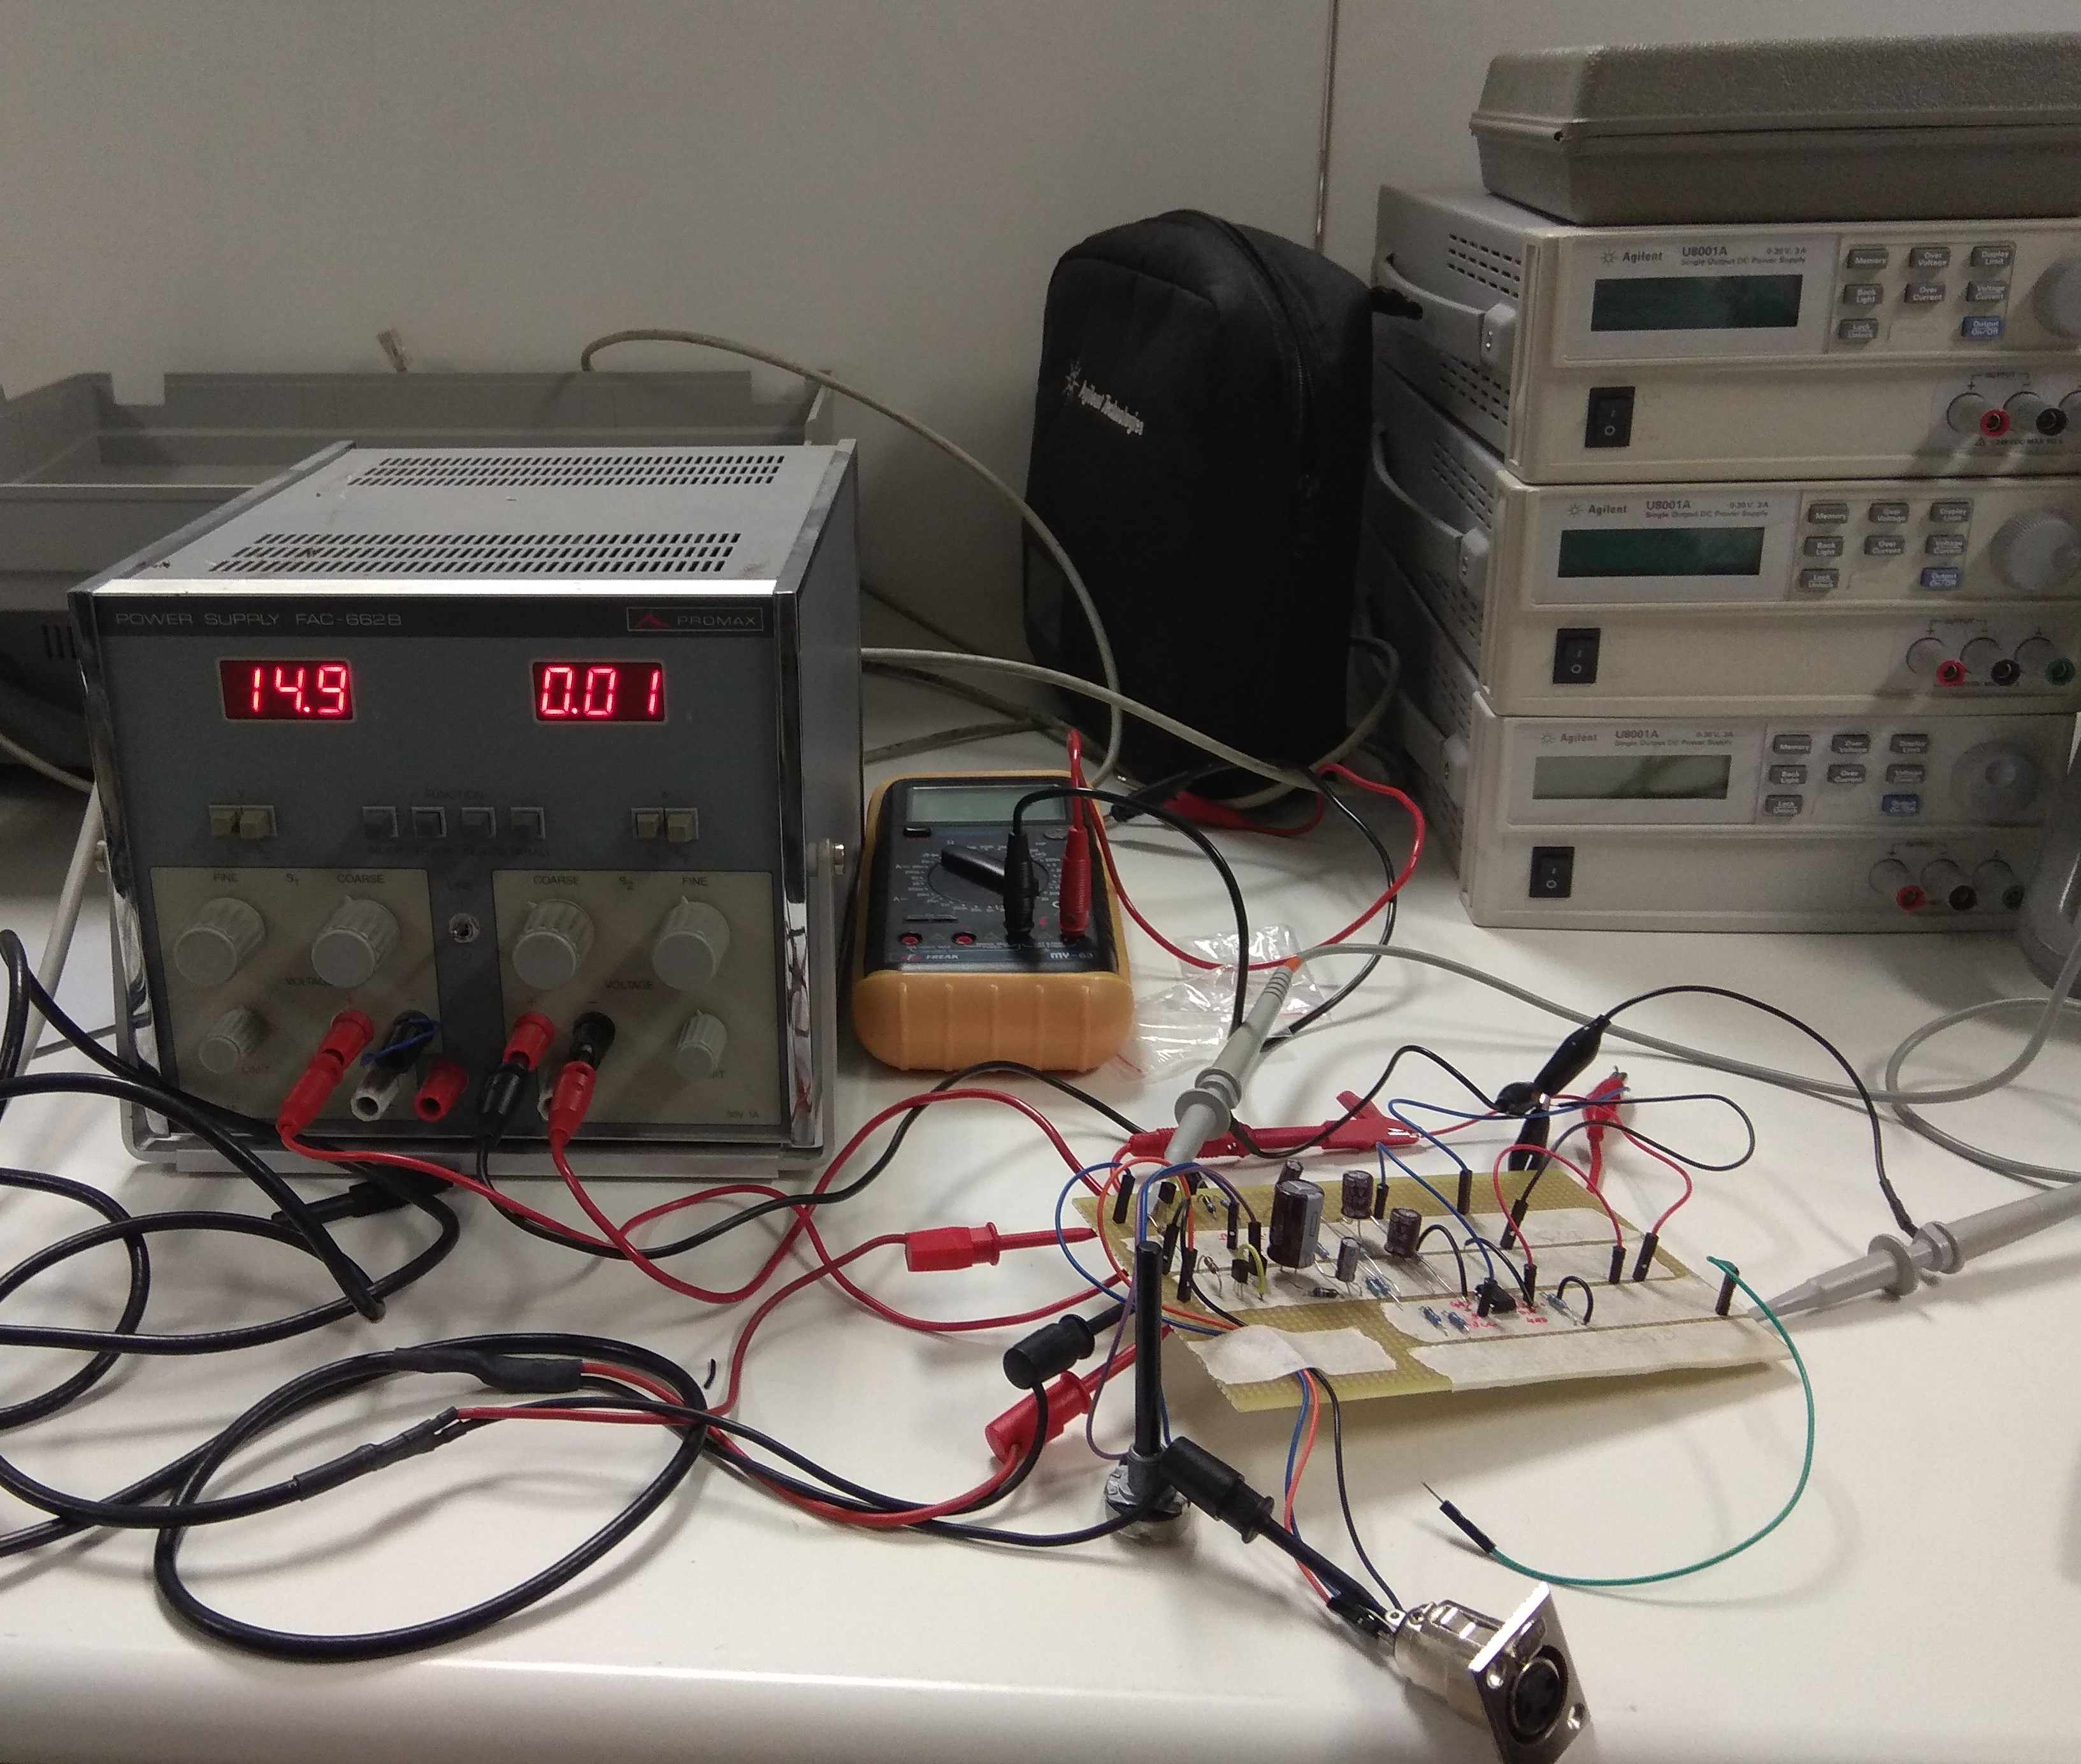
\includegraphics[width=10cm]{img/fuente.jpg}
\caption{\label{fig:fuente}Fuente de alimentación simétrica empleada}
\end{center}
\end{figure}

Normalmente, un pedal de efectos comercial precisa una alimentación de entre $\pm5$ y $\pm15V$ que se proporciona mediante un único transformador que posee varias salidas en paralelo. De esta forma se pueden alimentar todos los pedales de forma sencilla utilizando un único componente. Estos transformadores suelen tener un precio elevado debido a que deben ser muy robustos y silenciosos, ya que si no este se propaga por todos los pedales, introduciendo mucho ruido que luego va a ser amplificado produciendo un sonido desagradable y poco musical.


